\chapter{Экспериментальные методы исследования низкоразмерных наноструктур} \label{chapt2}

\section{Дифракция медленных электронов}
Дифракция электронов широко используется для исследования структуры 
поверхности. Информацию о структуре поверхности получают, анализируя
электроны, упруго рассеянные кристаллом. Интенсивность дифракционных
пучков содержит информацию о расположении атомов внутри элементарной 
ячейки. Распределение дифракционных пучков в пространстве дает 
информацию о решетке кристалла. Решетка прямо определяется из картины 
дифракции, так как эта картина однозначно связана с обратной решеткой
кристалл соотношением:
\begin{equation} \label{equation: reciprocal lattice vector}
	\textbf{k}-\textbf{k}_0 = \textbf{G}_{hkl}
\end{equation}
Здесь $\textbf{k}_0$ -- это вектор падающей волны, $\textbf{k}$ -- вектор
рассеянной волны, а $\textbf{G}_{hkl}$ -- вектор обратной решетки.


Для анализа структуры поверхности используется именно дифракция медленных
электронов, т.е. электронов низких энергий. Такой выбор энергии 
электронов обусловлен двумя основными причинами:
\vspace{15pt}
\begin{itemize}
	\item Во-первых, так как длина волны де-Бройля для электронов дается
	выражением $\lambda = \frac{h}{\sqrt{2mE}}$, то для типичных значений
	энергий электронов, используемых в ДМЭ ($30-200\si{\eV}$), длина 
	волны электрона составляет $~1-2\si{\angstrom}$, что удовлетворяет
	условию дифракции на атомных структурах, а именно, длина волны равна 
	или меньше межатомных расстояний.
	\item Во-вторых, средняя длина пробега таких низкоэнергетических
	электронов мала и составляет несколько атомных слоев. Поэтому 
	большинство упругих рассеяний происходит в самых верхних атомных
	слоях образца.
\end{itemize}
\vspace{15pt}
В результате, ДМЭ дает информацию в основном о двумерной структуре 
поверхности образца.


В случае дифракции на двумерной поверхности периодичность кристалла
в направлении, нормально поверхности, отсутствует, и~\ref{equation: reciprocal lattice vector}
становится
\begin{equation}
	\textbf{k}-\textbf{k}_0 = \textbf{G}_{hk}
\end{equation}


То есть закон сохранения импульса касается только компонент волновых
векторов, параллельных поверхности, а именно компоненты волнового
вектора рассеяния, параллельные поверхности, $\textbf{k}^{||}-\textbf{k}^{||}_0$ 
должны быть равны вектору двумерной обратной решетки поверхности $\textbf{G}_{hk}$.


На рис.~\ref{pic:evald} представлено построение Эвальда, модифицированное для случая
дифракции на двумерной решетки.
\begin{figure}[!ht]
\center{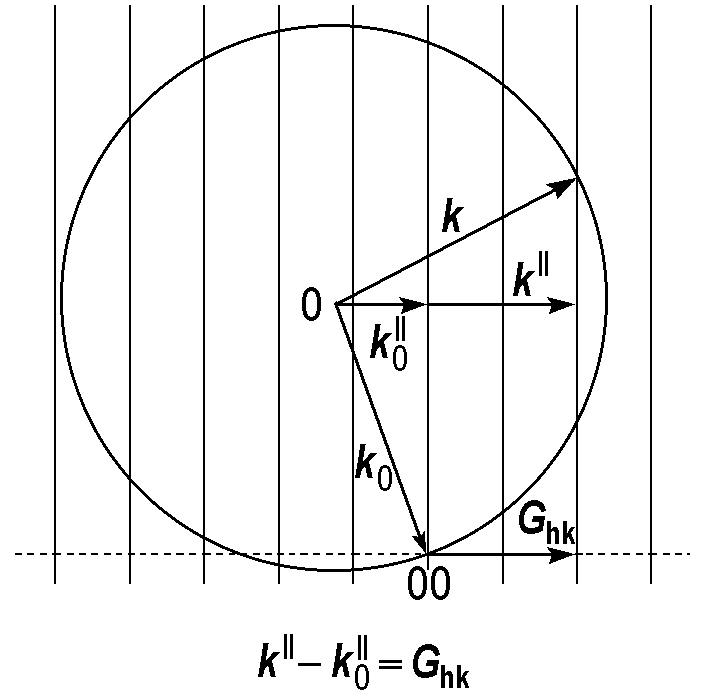
\includegraphics[width=0.4\linewidth]{evald.png}}
\caption{Построение Эвальда для дифракции на двумерной решетке 
поверхности.}
\label{pic:evald}
\end{figure}
В отличие от узлов трехмерной обратной решетки, здесь мы имеем дело 
со стержнями обратной решетки, которые проведены перпендикулярно 
поверхности через каждую точку двумерной обратной решетки.
Конец волнового вектора $\textbf{k}_0$ упирается в стержень обратной 
решетки. Пересечения стержней со сферой Эвальда определяют волновые 
векторы дифракционных пучков $\textbf{k}$.


Схема стандартной экспериментальной установки для прямого наблюдения
картин ДМЭ показана на рис.~\ref{pic:LEED_setup}(a).
	\begin{figure}[!ht]
		\center{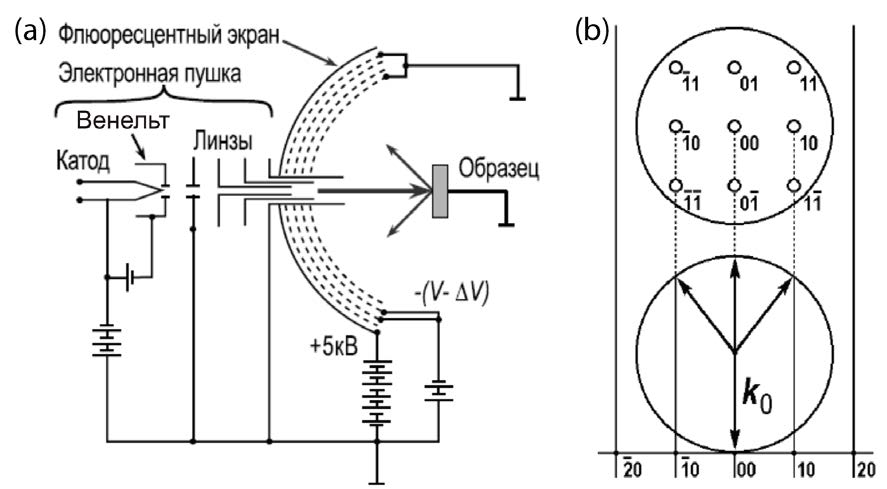
\includegraphics[width=0.7\linewidth]{leed_setup.png}}
		\caption{(a) Схема стандартной четырёх-сеточной установки для 
		наблюдения ДМЭ. (b) Обозначение дифракционных рефлексов на ДМЭ 
		картине при нормальном падении первичного пучка электронов. Рефлексы 
		имеют те же индексы, что и соответствующие узлы двумерной обратной 
		решётки.}
		\label{pic:LEED_setup}
	\end{figure}
Основные элементы установки -- это
	\vspace{15pt}
		\begin{itemize}
			\item Электронная пушка, генерирующая коллимированный пучок 
			электронов низких энергий;
			\item Держатель образца с исследуемым образцом;
			\item Полусферический флюоресцентный экран с набором из четырех 
			сеток для наблюдения картины дифракции упруго рассеянных электронов.
		\end{itemize} 
	\vspace{15pt}
Рассеянные на поверхности электроны проходят через задерживающую сетку,
отсекающую вторичные и неупруго рассеянные электроны, ускоряются и 
сталкиваются с флуоресцентным экраном, вызывая его свечение, 
детектируемое CCD-камерой.


Сравнение геометрии ДМЭ установки и построения Эвальда показывает, 
что картина дифракции, наблюдаемая на экране, соответствует обратной 
решётке поверхности. Трансляционные векторы обратной решетки 
$\textbf{b}_i$ связаны с векторами кристаллической решетки поверхности
$\textbf{a}_i$ выражениям
	\begin{equation}
		\textbf{b}_1=2\pi\frac{\textbf{a}_2\times\textbf{n}}{|\textbf{a}_1\times\textbf{a}_2|},\quad\textbf{b}_2=2\pi\frac{\textbf{n}\times\textbf{a}_1}{|\textbf{a}_1\times\textbf{a}_2|}
	\end{equation}
где \textbf{n} -- нормаль к поверхности.
Наблюдаемые рефлексы индексируются также, как и 
узлы обратной решетки, а именно величинами $h$, $k$. Зеркальный рефлекс
принято приписывать к точке $(0,0)$. При нормальном падении первичного
пучка электронов он находится в центре картины ДМЭ рис.~\ref{pic:LEED_setup}(б).


Для анализа картины ДМЭ сначала качественно оценивают структурное
совершенство изучаемой поверхности. От хорошо упорядоченной поверхности
наблюдается картина ДМЭ с яркими четкими рефлексами и низким уровнем
фона. Присутствие структурных дефектов приводит к тому, что рефлексы
становятся менее интенсивными и более размытыми, а уровень фона 
возрастает. Отсутствие каких-либо рефлексов на картине ДМЭ указывает
на то, что поверхность разупорядоченная (аморфная или мелкодисперсная
поликристаллическая).


Следующий шаг заключается в рассмотрении геометрического расположения
рефлексов. ДМЭ картина типа $1\times1$ представляет наиболее простой
случай. Очевидно, что поверхность, имеющая структуру нижележащих 
плоскостей подложки, дает именно такую картину.


Если на поверхности образуется сверхструктура, то в дифракционной 
картине появляются новые рефлексы. Эти рефлексы называют 
дополнительными, чтобы отличать их от основных рефлексов, образующих
картину $1\times1$.


Таким образом, ДМЭ позволяет быстро характеризовать качество полученных
пленок адсорбата и определять параметры обратной решетки поверхности 
из геометрии дифракционной картины.






\section{Рентгеновская фотоэлектронная спектроскопия} \label{method_XPS}

Одним из самых мощных и информативных инструментов для изучения 
энергетического спектра заполненных электронных состояний вещества
является фотоэлектронная спектроскопия. Она делится на две методики,
отличающиеся задачами исследования и энергиями фотонов:
	\vspace{15pt}
		\begin{itemize}
			\item \textit{Рентгеновская фотоэлектронная спектроскопия}(РФЭС) 
			применяется в основном для анализа остовных электронных уровней,
			поэтому используется рентгеновское излучение в диапазоне энергий
			фотонов около $100-10 000 \si{\eV}$.
			\item \textit{Ультрафиолетовая фотоэлектронная спектроскопия}(УФЭС),
			используется преимущественно для анализа состояний валентной зоны. Для нее характерны энергии фотонов $10-100 \si{\eV}$.
		\end{itemize}
	\vspace{15pt}


В настоящей работе использовалась методика рентгеновской 
фотоэлектронной спектроскопии, с помощью которой были изучены остовные
электронные уровни системы h-BN/Co(0001) при взаимодействии с 
молекулярным кислородом.

\paragraph{Фотоэффект.}
В основе фотоэлектронной спектроскопии лежит фотоэлектрический эффект.
Если электрон, первоначально находившийся в состоянии с энергией
связи $E_i$, поглощает фотон с энергией $\hbar\omega$ и покидает 
твердое тело, то такой электрон называется фотоэлектроном, а его
кинетическую энергию, с которой он покидает твердое тело, можно записать
в виде
	\begin{equation}
		E_{kin}=\hbar\omega-E_i-\phi,
	\end{equation}

где $\phi=E_{vacuum}-E_{Fermi}$ -- работа выхода материала рис.~\ref{pic:XPS_diagram}.
	\begin{figure}[!ht]
		\center{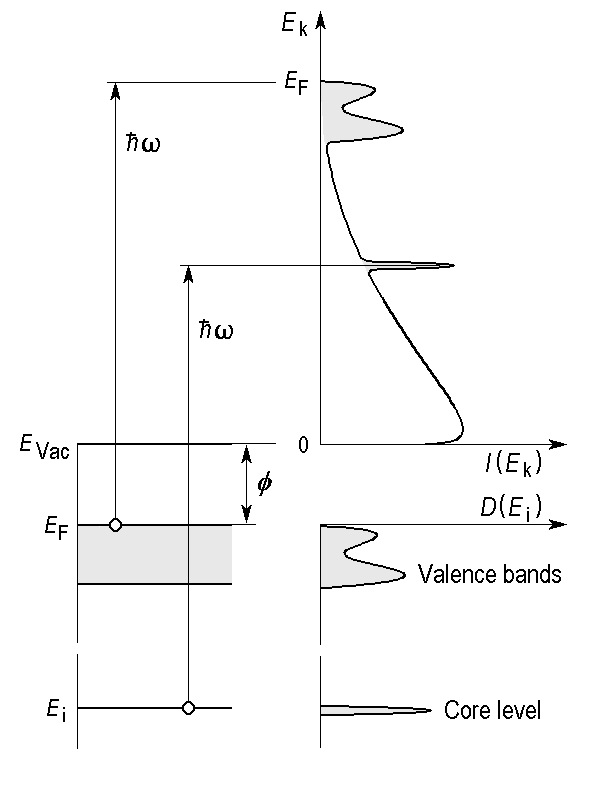
\includegraphics[width=0.5\linewidth]{xps_pic.png}}
		\caption{Схематическая диаграмма, иллюстрирующая процесс фотоэмиссии
		на поверхности металла.}
		\label{pic:XPS_diagram}
	\end{figure}


Для того, чтобы зарегистрировать фотоэлектрон, должны быть выполнены
следующие условия:
	\vspace{15pt}
		\begin{itemize}
			\item Энергия фотона должна быть достаточна, чтобы электрон смог
			покинуть твердое тело, то есть $\hbar\omega\geq E_i+\phi$.
			\item Скорость электрона должна быть направлена в сторону внешней 
			поверхности.
			\item Электрон не должен потерять энергию в столкновениях с другими
			электронами на своем пути к поверхности.
		\end{itemize}
	\vspace{15pt}


\paragraph{Трехступенчатая модель фотоэмиссии.}
Фотоэмиссию часто описывают в рамках трехступенчатой модели~\cite{Hufner2019},
где процесс фотоэмиссии разбивается на три независимые части:
	\vspace{15pt}
		\begin{enumerate}
			\item Поглощение кванта с образованием фотоэлектрона.
			\item Движение электрона к поверхности твердого тела.
			\item Выход возбужденных электронов в вакуум.
		\end{enumerate}
	\vspace{15pt}


1) На первом шаге происходит возбуждение фотоэлектронов.
Электрон поглощает фотон и, за счет полученной энергии, переходит из
невозбужденного $E_i, \textbf{k}_i$  в возбужденное состояние выше 
уровня ферми $E_f, \textbf{k}_f$. Вероятность такого перехода 
определяется золотым правилом Ферми:
	\begin{equation} 
		\label{Fermi_rule}
		w_{fi}=\frac{2\pi}{\hbar}|\left\langle\psi_f,\textbf{k}_f|H^{int}|
		\psi_i,\textbf{k}_i\right\rangle|^2\delta(E_f-E_i-\hbar\omega)
	\end{equation}
Здесь $\psi_i$ -- волновая функция, $E_i$ -- энергия начального состояния
фотоэлектрона, а  $\psi_f$ и $E_f$ -- волновая функция и энергия 
конечного состояния соответственно. Дельта функция $\delta(E_f-E_i-\hbar\omega)$
отражает закон сохранения энергии. Гамильтониан $H^{int}$ взаимодействия
электрона и электромагнитного поля может быть записан как
	\begin{equation} 
	\label{equation:hamiltonian}
		H^{int}=\frac{1}{2mc}(\textbf{A}\cdot\hat{\textbf{p}}+\hat{\textbf{p}}\cdot\textbf{A})
	\end{equation}
где $\hat{\textbf{p}}$ -- оператор импульса и $\textbf{A}$ -- векторный потенциал электромагнитного поля. Для бесспиновой частицы гамильтониан
\ref{equation:hamiltonian} может быть приведен к виду
	\begin{equation} 
		\label{equation:hamiltonian}
		H^{int}=\frac{1}{mc}(\textbf{A}\cdot\hat{\textbf{p}})
	\end{equation}
Если представить векторный потенциал \textbf{A} в виде разложения по
плоским волнам, можно показать, что матричный элемент перехода
будет пропорционален
	\begin{equation} 
		\label{equation:spinless_electron_hamiltonian}
		\left\langle\psi_f,\textbf{k}_f|H^{int}|
		\psi_i,\textbf{k}_i\right\rangle\sim
		\left\langle\psi_f,\textbf{k}_f|\textbf{ep}e^{i\textbf{k}r}|
		\psi_i,\textbf{k}_i\right\rangle
	\end{equation}
где \textbf{e} -- это вектор поляризации, а \textbf{k} -- волновой вектор
падающего излучения. В длинноволновом (дипольном) приближении $e^{i\textbf{k}r}\rightarrow 1$, 
тогда вероятность перехода становится пропорциональна
$\left\langle\psi_f,\textbf{k}_f|\textbf{ep}|\psi_i,\textbf{k}_i\right\rangle$. Также в этом приближении для гамильтониана
\ref{equation:spinless_electron_hamiltonian} можно вывести 
правила Лапорта для орбитального и спинового квантовых чисел:
$\Delta\l=\pm1,\ \Delta$$S=0$.


2) На втором шаге трехступенчатой модели фотоэмиссии возбужденный
фотоэлектрон проходит через твердое тело на поверхность. В течение 
этого перемещения, фотоэлектрон может испытывать рассеяние при 
взаимодействии с фононами или другими электронами. Упруго рассеянные
фотоэлектроны от нерассеянных различаются по времени, которое они 
тратят на достижение поверхности, и направлению волнового вектора. 
Неупруго рассеянные фотоэлектроны теряют энергию в процессе рассеяния
и достигают поверхности с куда меньшей энергией, чем упруго рассеянные.
Такие электроны называют вторично рассеянными. 
Расстояние, которое преодолевает электрон в твердом теле до первого 
рассеяния, называется длиной свободного пробега и является функцией 
энергии $\lambda(E)$. Длина свободного пробега не зависит от материала.
Кривая зависимости глубины выхода электрона от кинетической энергии для нескольких различных элементов показана на рис.~\ref{pic:mean_free_path}.
	\begin{figure}[!ht]
		\center{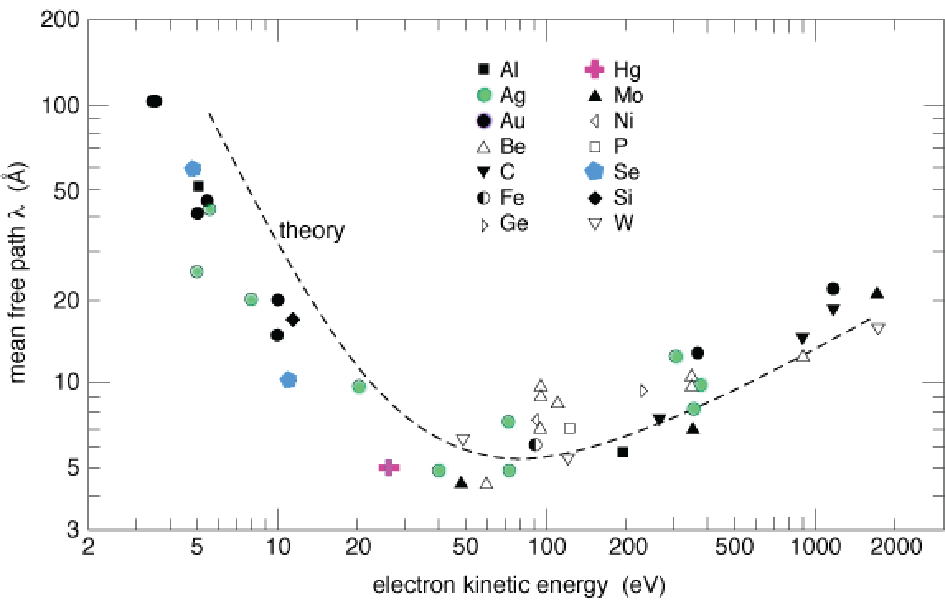
\includegraphics[width=0.7\linewidth]{mean_free_path.png}}
		\caption{Набор экспериментальных данных для длин свободного пробега 
		электронов в различных материалах, представленных в виде зависимости 
		от кинетической энергии электронов~\cite{Mean_Free_Path}.}
		\label{pic:mean_free_path}
	\end{figure}
Медленные электроны с энергией $<10\si{\eV}$ слабо 
взаимодействуют с фононами и электронами и поэтому проходят большие
дистанции. Минимум $\lambda(E)$ приходится на энергии $30-200\si{\eV}$.
На этих энергиях вероятность рассеяния электрона увеличивается, в
основном, за счет неупругого взаимодействия и возбуждения плазмонов.
Для быстрых высокоэнергетических электронов с энергией $>200\si{\eV}$
эффективное сечение рассеяния уменьшается, в результате чего $\lambda(E)$ растет.


3) На третьем шаге трехступенчатой модели фотоэмиссии электроны,
достигшие поверхности твердого тела, должны преодолеть потенциальный
барьер высотой $eV_0=E_{vac}-E_0$ между наивысшим заполненным уровнем
и уровнем вакуума~\ref{pic:final_state_photoemission}(a). 
	\begin{figure}[!ht]
		\center{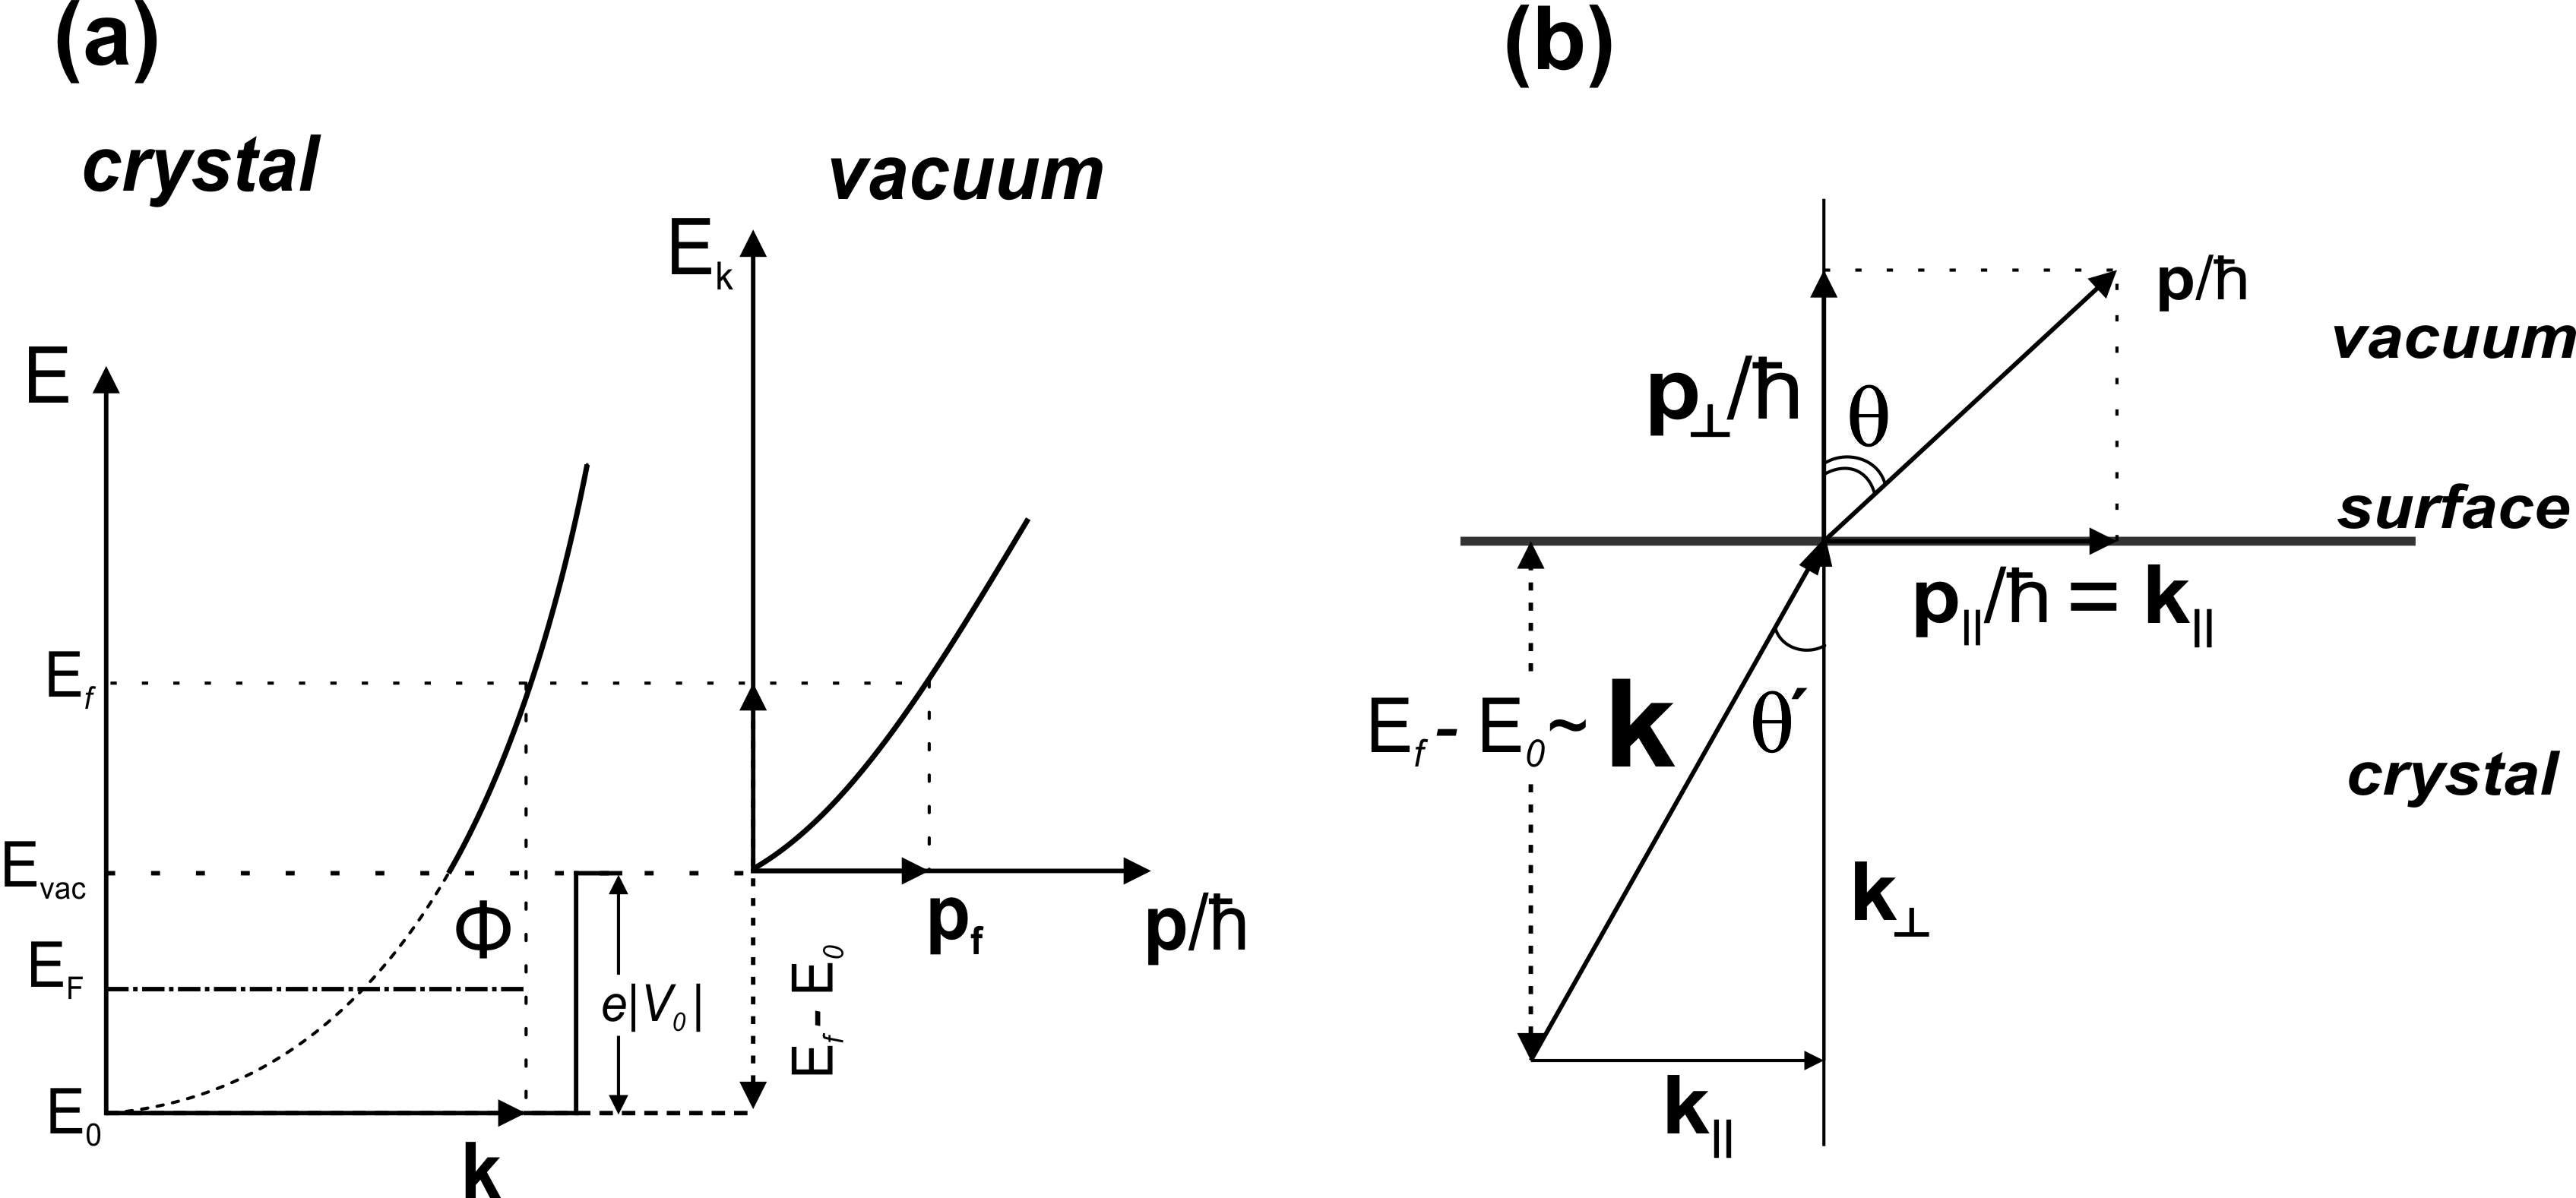
\includegraphics[width=0.7\linewidth]{final_state_photoemission.png}}
		\caption{Схематическая иллюстрация финальной стадии фотоэмиссии(a), 
		Закон Снеллиуса для фотоэлектронов(b).}
		\label{pic:final_state_photoemission}
	\end{figure}
При переходе через поверхность параллельная составляющая вектора 
электрона сохраняется (т.к. ничего не влияет на эту величину), а 
перпендикулярная составляющая уменьшается на величину, определяемую 
внутренним потенциалом кристалла (в вакууме кинетическая энергия 
отсчитывается от уровня вакуума, а в твёрдом теле -- от дна 
“потенциального ящика”, глубина которого определяется внутренним 
потенциалом). Это приводит к преломлению электронной волны на выходе 
из кристалла~\ref{pic:final_state_photoemission}(b).


\paragraph{Анализ атомного состава с помощью РФЭС.} 
РФЭС может быть использована для определения атомного состава образца.
В основе количественного анализа химического состава образца с 
помощью РФЭС лежат следующие предположения:
	\vspace{15pt}
		\begin{itemize}
			\item Поверхность образца идеально плоская;
			\item Исследуемый образец является поликристаллическим или
			аморфным, или же влияние кристаллической структуры на угловое
			распределение фотоэлектронов пренебрежимо мало;
			\item Ослабление пучка фотоэлектронов при движении в твердом теле
			имеет экспоненциальную зависимость от пройденного пути;
			\item Поверхностным отражением и преломлением можно пренебречь.
		\end{itemize}
	\vspace{15pt}
В случае пренебрежения упругим рассеянием фотоэлектронов, выражение
для интенсивности фотоэлектронной линии тонкого монослоя:
	\begin{equation}
		I=nf\frac{d\sigma_{nl}(h\nu,\gamma)}{d\Omega}AT(E_k),
	\end{equation}
где $E_k$ -- кинетическая энергия фотоэлектронов, формирующих пик, 
\textit{n} -- концентрация атомов, \textit{f} -- поток фотонов,
$\frac{d\sigma_{nl}(h\nu,\gamma)}{d\Omega}$ -- дифференциальное
сечение фотоионизации, \textit{A} -- площадь области анализа, $T(E_k)$ -- 
функция пропускания спектрометра.



Также РФЭС спектр содержит информацию о химическом состоянии атомов
составляющих поверхность. Точные измерения энергетического положения 
остовного уровня для данного элемента показывают, что положение уровня 
меняется в зависимости от химического состояния атома, которое зависит 
от типа атомов окружения и характера химического связывания с ними.
Такие смещения называют химическими сдвигами.
Химический сдвиг относительно его положения в нейтральном атоме может 
быть как положительным, так и отрицательным и изменяться в пределах
нескольких $\si{\eV}$. Объяснить природу химического сдвига 
в простейшем случае можно следующим образом:
	\vspace{15pt}
		\begin{itemize}
			\item Энергия связи электронов состоит из двух основных вкладов: 
			кулоновского притяжения к ядру и межэлектронного взаимодействия.
			\item В результате образования химической связи происходит 
			перераспределение плотности валентных электронов взаимодействующих
			атомов, следствием этого является изменение химического состояния
			атома и его энергии связи.
			\item При увеличении заряда на данном атоме происходит усиление
			электронного экранирования, в связи с чем связь электрона ослабевает.
			В противоположном случае, при уменьшении заряда, электронное
			экранирование ослабевает, и энергия связи увеличивается.
		\end{itemize}
	\vspace{15pt}
Если химсдвиг $<0.5\si{\eV}$, то оказывается невозможным
его определить "на глаз". В этом случае необходимо многокомпонентный
пик разложить на отдельные компоненты. Форма остовной линии 
представляет собой свёртку Лоренциана
	\begin{equation} 
		\label{equation: Lorenc}
		L_h(E)=\frac{1}{\pi \beta}\left(1+\left[\frac{E}{\beta}\right]^2\right)^{-1},
	\end{equation}
обусловленного конечным временем жизни возбуждённого состояния атома, 
и Гауссиана
	\begin{equation}
		G_h(E)=exp\left(-\ln{2\left[\frac{E}{\beta}\right]^2}\right),
	\end{equation}
ширина которого определяется главным образом инструментальным 
разрешением. 


Продуктом асимметрии Гауссиана и Лоренциана одинаковой ширины
и высоты является
	\begin{equation}
		GL_p(E)=\left(1+M\left[\frac{E}{\beta+\alpha E}\right]^2\right)^{-1}
		exp\left(-(1-M)\ln{2\left[\frac{E}{\beta+\alpha E}\right]^2}\right),
	\end{equation}
где $\alpha\geq0$ -- асимметрия, $M$ -- смешанное отношение от 0 
(чистый Гауссиан) до 1 (чистый Лоренциан).


Сумма асимметрии Гаусииана и Лоренциана одинаковой ширины и высоты:
	\begin{equation}
		GL_s(E)=\left(1+M\left[\frac{E}{\beta+\alpha E}\right]^2\right)^{-1}
		+(1-M)
		exp\left(-\ln{2\left[\frac{E}{\beta+\alpha E}\right]^2}\right).
	\end{equation}


В настоящей работе при разложении спектров фотоэмиссии использовались
именно эти формулы.



\section{Спектроскопия поглощения рентгеновских лучей}

Спектроскопия, основанная на изучении ближней тонкой структуры 
рент­геновских спектров поглощения (БТСРСП или NEXAFS: Near-Edge 
X-ray Absorbtion Fine Structure), позволяет изучать свободные 
состояния зоны про­водимости~\cite{Stohr1992}. В этом методе, в 
зависимости от энергии фотонов в окрестности края поглощения,
измеряется коэффициент поглощения рентгеновских лучей.
	\begin{figure}[!ht]
		\center{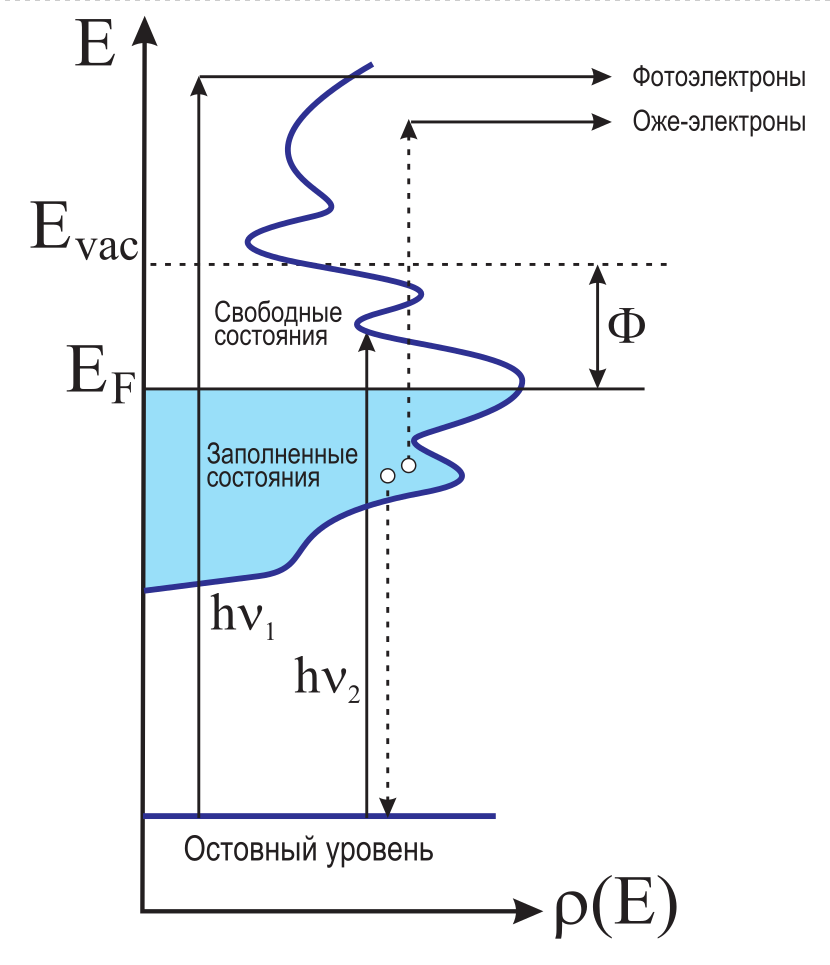
\includegraphics[width=0.5\linewidth]{NEXAFS_pic.png}}
		\caption{Спектроскопия NEXAFS: упрощенная энергетическая диаграмма.}
		\label{pic:NEXAFS_diagram}
	\end{figure}
В процессе фотовозбуж­дения электрон переходит из начального состояния \textit{i} в конечное состояние \textit{f}, как это уже упоминалось в разделе \ref{method_XPS}.
На диаграмме рис.~\ref{pic:NEXAFS_diagram} показано, что остовный уровень
соответствует начальному состоянию, а конечное стостояние лежит в зоне 
проводимости. Так как остовный уровень характеризуется фиксированным значением энергии, то появляется возможность задавать энергию конечного состояния в соот­ветствии
с законом сохранения энергии $E_f=E_i+h\nu$, при помощи выбора $h\nu$
вблизи края поглощения. 

Экспериментально спектроскопия поглощения может быть реализована разными
способами. В настоящей работе использовался метод измерения полного квантового выхода 
электронов (TEY: TolalElectron Yield) – среднего числа электронов, выбиваемых из образца одним фо­тоном. Так как выходу электронов всегда предшествует
поглощение фотонов, то 
зависимость полного выхода от энергии фотонов слабо отличается от
зависимости коэффициента поглощения. В этом случае возможна эмиссия электронов. Примеры таких процессов
показаны на рис.\ref{pic:NEXAFS_diagram}.
% Если энергии фотонов $h\nu_2$ недостаточно для прямого вы­хода
% фотоэлектрона в вакуум, то возможна эмиссия в результате Оже-процесса
% с участием электронов валентной зоны. Если же энергия фотона $h\nu_1$ достаточ­но
%  высока, то возможен как Оже процесс, так и прямой выход фотоэлектрона
% из твердого тела. Необходимо отметить, что спектроскопия полного квантово­
% го выхода, является поверхностно-чувствительным методом, но глубина анализа
% обычно больше, чем в фотоэлектронной спектроскопии, и составляет несколько
% нанометров. Причиной является то, что значительный вклад в полный выход
% дают вторичные электроны, выходящие с большей глубины, чем первичные фо­тоэлектроны.

Полный квантовый выход пропорционален интенсивности излучения, а так­же
току через образец. Поэтому для измерений используется пикоамперметр.
Источником фотонов является канал вывода СИ, обеспечивающий возможность
изменения энергии рентгеновского излучения, а также измерения потока фото­нов.


% Использование излучения с линейной поляризацией расширяет возможно­
% сти анализа многих систем с $sp^2$ гибридизацией, включая графен. В частности,
% измерение зависимости спектров NEXAFS от направления вектора поляриза­ции
% фотонов относительно поверхности графена дает возможность выделить в
% спектрах вклады, соответствующие переходам в $\pi$- или $\sigma$-состояния зоны 
% про­водимости~\cite{Stohr1992}. Так как $\pi$-орбитали направлены перпендикулярно 
% поверхно­сти, а $\sigma$ – параллельно, то соответствующие им участки спектра поглощения
% проявляют различную зависимость коэффициента поглощения от угла между
% вектором поляризации и поверхностью. При поляризации вдоль поверхности,
% переходы в $\pi$-состояния запрещены, а переходы в $\sigma$-состояния достигают
% мак­симальной вероятности.